% document class using the Springer publishing company's document class
\documentclass[envcountsame,envcountchap]{svmono}

% packages to include additional functionality
\usepackage{makeidx}         % allows index generation
\usepackage{graphicx}        % standard LaTeX graphics tool
                     	       % when including figure files
\usepackage{multicol}        % used for the two-column index
\usepackage[bottom]{footmisc}% places footnotes at page bottom
\usepackage{wrapfig} % for wrapping images with text
\usepackage{color} % for coloring links
\usepackage{fancyvrb}
\usepackage{amssymb} %for symbols like arrows
\usepackage{listings} %for inserting code 
\usepackage{pdfpages} %to insert pdf
\usepackage[hyphens]{url}
\usepackage{hyperref} %to insert url
\usepackage{nameref}
\begin{document}
\author{Srividya Majeti}
\title{Assignment 4}

\subtitle{CS 532:  Introduction to Web Science\\Dr. Michael Nelson\\Spring 2016}

% note that this special command is part of the document class
% and, in addition to creating the title page, also inserts the 
% current date on the page
\maketitle

\frontmatter

\tableofcontents

\mainmatter

% include other tex files so we don't have one huge document to scroll through
\chapter{Question 1}
\label{intro}

\textbf{Demonstrate that you know how to use ``curl'' well enough to correctly POST data to a form. Show that the HTML response that is returned is ``correct''.  That is, the server should take the arguments you POSTed and build a response accordingly.  Save the HTML response to a file and then view that file in a browser and take a screen shot.}\\

To POST data to a form using cURL, I did the following:
\begin{itemize}
\item I created a form using PHP with name as an input element and a submit button.

\item When we open this PHP form in the browser and type any name, it displays a response saying ``Welcome followed by the text''.

\item By using the following cURL command we can POST data to the form which is received by the server and generates a response with the same message that we see on the browser. By using -o followed by parameter, I am outputting the HTML response to a file.
\end{itemize}
\begin{verbatim}
 curl -d name=Srividya ``www.cs.odu.edu/~smajeti/postForm.php'' 
 -o output.html
\end{verbatim}


\newpage

\lstinputlisting[language=PHP,caption=``PHP script'',frame=single,breaklines=true,captionpos=b,numbers=left,showspaces=false,showstringspaces=false,basicstyle=\footnotesize]{src/postForm.php}

\begin{figure}[h!]
\begin{center}


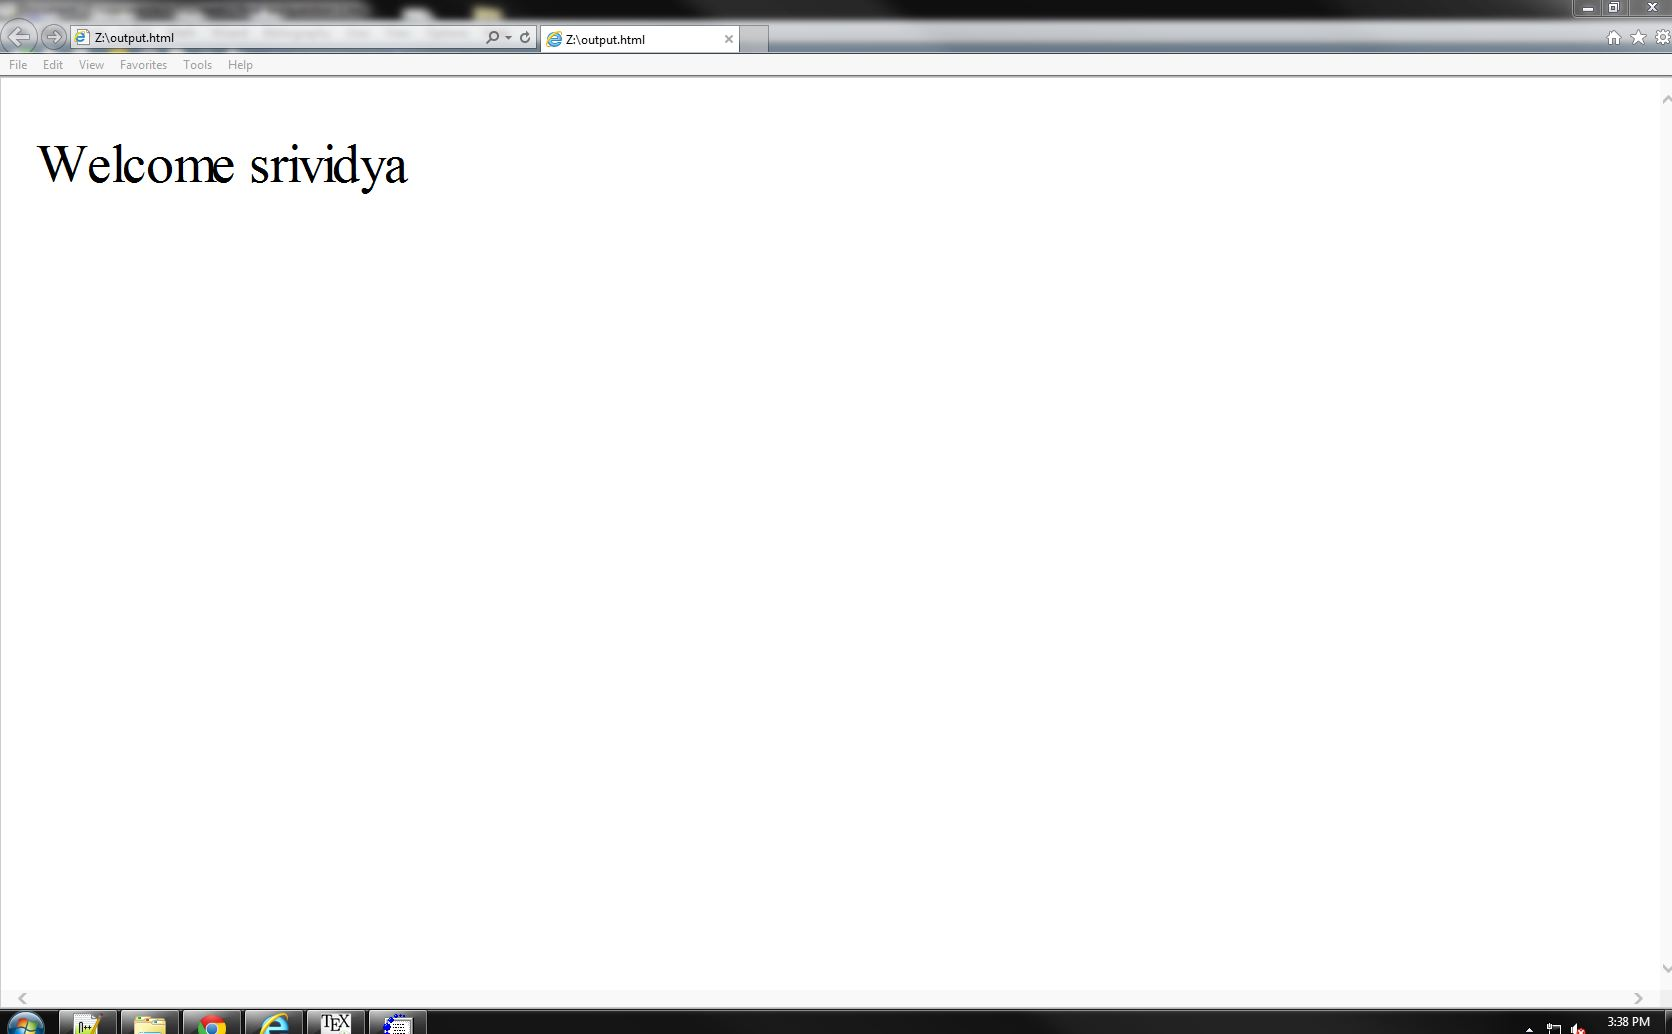
\includegraphics[scale=0.30, keepaspectratio=true]{figures/q1screenshot.JPG}
\caption{HTML response saved into a file and viewed in browser.}
\label{mcpon_navy_mil}
\end{center}
\end{figure}

\chapter{Question 2}
\label{avoiding-uri-aliases} 

\textbf {Determine if the friendship paradox holds for your Twitter account. Since Twitter is a directed graph, use ``followers'' as value you measure
(i.e., ``do your followers have more followers than you?'').\\
Generate the same graph as in question 1, and calcuate the same  mean, standard deviation, and median values.\\
For the Twitter 1.1 API to help gather this data, see:}\\
{\url{https://dev.twitter.com/docs/api/1.1/get/followers/list}}\\
\textbf{If you do not have followers on Twitter (or don't have more than 50), then use my twitter account ``phonedude\textunderscore mln''.}

Following are the steps that I have taken to solve this problem:
\begin{itemize}
\item I did not have more than 50 followers, so I randomly picked a user with the screen name `ohttic' from your followers list. He has 258 Followers and is following 1,923 people.
\item Twitter provides an API to get the list of followers. This API returns an object of followers with the profile information. `Tweepy' library is a wrapper around Twitter that makes it easier to retrieve Twitter data. I used this library to get the followers data.
\item I iterated through the list of users and retrieved the `screen\textunderscore name', `followers\textunderscore count' and `friends\textunderscore count'. I stored this information in a JSON structure and saved it into a file `userFollowerdata' . This code is listed in Listing \ref{lst:q2code1}.
\item Furthermore, I extracted the followers count from the JSON and stored it in a file `followersCount'. This code is listed in Listing \ref{lst:q2code2}
\item I calculated the mean, median and standard deviation for the followers count. This code is listed in Listing \ref{lst:q2code3}. The mean, median and standard deviation are given in Table \ref{Table:q2table1}

\begin{table}

\caption{Mean, Median and Standard Deviation of number of followers of followers}
\label{Table:q2table1}
\begin{center}
\begin{tabular}{| c | c |}
\hline
Key & Value \\ \hline

Mean & 54474.2 \\ \hline
Median & 5477.0 \\ \hline
Standard Deviation & 120893.613437 \\ \hline

\hline

\end{tabular}
\end{center}
\end{table}

\newpage
\item Figure \ref{fig:q2fig2} illustrates the ranking of `ohttic' in terms of followers count in comparison with his followers.
\begin{figure}[h!]
\begin{center}
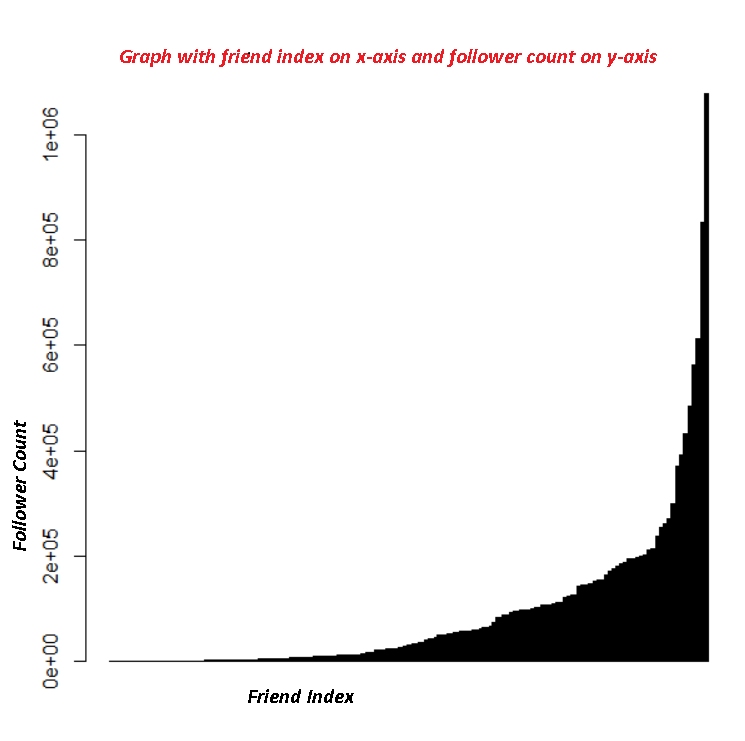
\includegraphics[scale=0.55, keepaspectratio=true]{figures/followerWithoutLog.PNG}
\caption{Graph with number of followers on y-axis and followers on x-axis }
\label{fig:q2fig2}
\end{center}
\end{figure}

\begin{figure}[h!]
\begin{center}
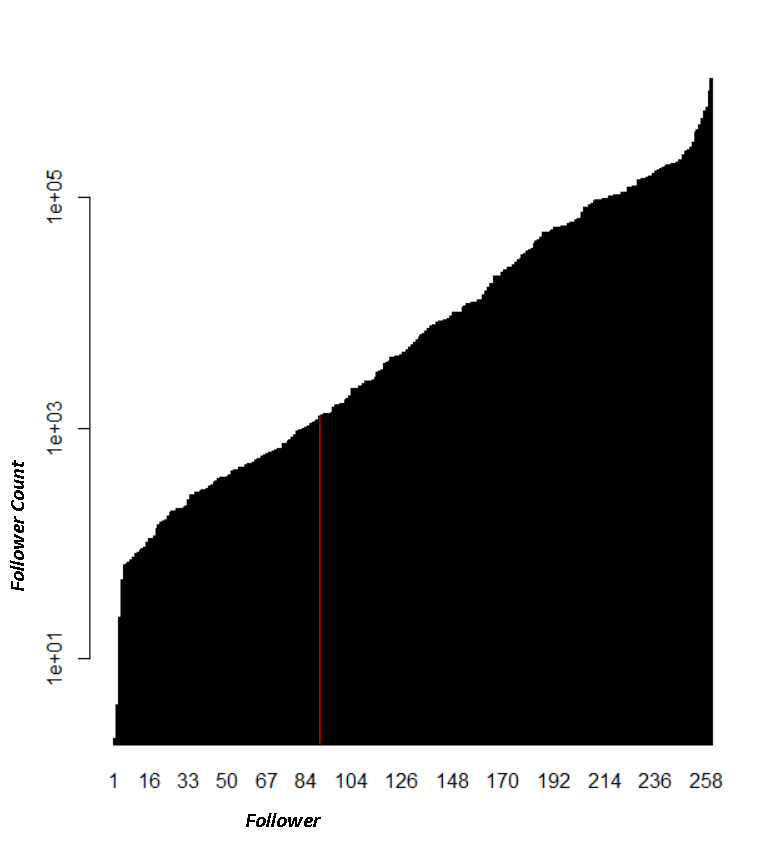
\includegraphics[scale=0.55, keepaspectratio=true]{figures/finalFollower.PNG}
\caption{Graph with number of followers on y-axis in log scale and followers on x-axis }
\label{fig:q2fig3}
\end{center}
\end{figure}
\newpage
\item From the calculated median value `5477.0' and number of followers `ohttic' have `258' we can say that he have less number of followers than his followers.

\end{itemize}

\newpage
\textbf{Code Listing}
\lstinputlisting[language=Python,caption=Python code for retrieving friends data and storing screenName followersCount and friendsCount in a JSON structure ,frame=single,label=lst:q2code1,breaklines=true,captionpos=b,numbers=left,showspaces=false,showstringspaces=false,basicstyle=\footnotesize]{src/getFollowerAndFriendsData.py}

\newpage
\textbf{Code Listing}
\lstinputlisting[language=Python,caption=Python code for extracting followers count from JSON structure,frame=single,label=lst:q2code2,breaklines=true,captionpos=b,numbers=left,showspaces=false,showstringspaces=false,basicstyle=\footnotesize]{src/extractFollowers.py}

\textbf{Code Listing}
\lstinputlisting[language=Python,caption=Python code for calculating mean median and standard deviation,frame=single,label=lst:q2code3,breaklines=true,captionpos=b,numbers=left,showspaces=false,showstringspaces=false,basicstyle=\footnotesize]{src/getMeanMedianStandardDeviation2.py}
%\chapter{Extra-Credit Question 3}
\label{available-representation}

\textbf{Repeat question 1, but with your LinkedIn profile.}

\begin{itemize}
\item  To find the page rank for all the 10 URIs I used a free PR estimator on the web which is located at: \\
{\url{http://www.seocentro.com/tools/search-engines/pagerank.html}}. 
\item The URI and its page rank is summarized in the Table \ref{Table:q3table1}.
\item While finding the page rank for each URI I took a screenshot. The screenshits are in the Figures \ref{fig:q3fig1},  \ref{fig:q3fig2},  \ref{fig:q3fig3},  \ref{fig:q3fig4},  \ref{fig:q3fig5},  \ref{fig:q3fig6},  \ref{fig:q3fig7},  \ref{fig:q3fig8} \ref{fig:q3fig9},  \ref{fig:q3fig10}
\end{itemize}

Comparing the rankings in question 2 and 3 I observed that their is a lot of difference in rankings. The reason behind this difference is, when we rank the URIs based on TF, IDF and TFIDF, we look for the frequency of the term. But the PR estimator ranks the URIs based on the quality of the document and also the quantity of backlinks. Calculating pagerank based on frequency of the term is not a good idea because even a poor quality document with high query term frequency will be ranked high. 


\chapter{Extra-Credit Question 4}
\label{available-representation}

\textbf{Repeat question 2, but change ``followers'' to ``following''?  In other words, are the people I am following following more people?}

\begin{itemize}
\item Using the `userFollowerData' file generated in question 2 as input, I extracted the following \textunderscore count from the JSON structure and stored it in a file `followingCount'. This code is listed in Listing \ref{lst:q4code1}
\item I calculated the mean, median and standard deviation for the following count. This code is listed in Listing \ref{lst:q4code2}. The output of mean, median and standard deviation are given in Table \ref{Table:q4table1}

\begin{table}

\caption{Mean, Median and Standard Deviation of number of people followed by the people followed by `ohttic'}
\label{Table:q4table1}
\begin{center}
\begin{tabular}{| c | c |}
\hline
Key & Value \\ \hline

Mean & 45183.2 \\ \hline
Median & 4609.5 \\ \hline
Standard Deviation & 96280.5156542 \\ \hline

\hline

\end{tabular}
\end{center}
\end{table}

\newpage
\item I created a graph with following count on y-axis and the friends themselves on x-axis including `ohttic'. The graph is summarized in Figure \ref{fig:q4fig2}.
\begin{figure}[h!]
\begin{center}
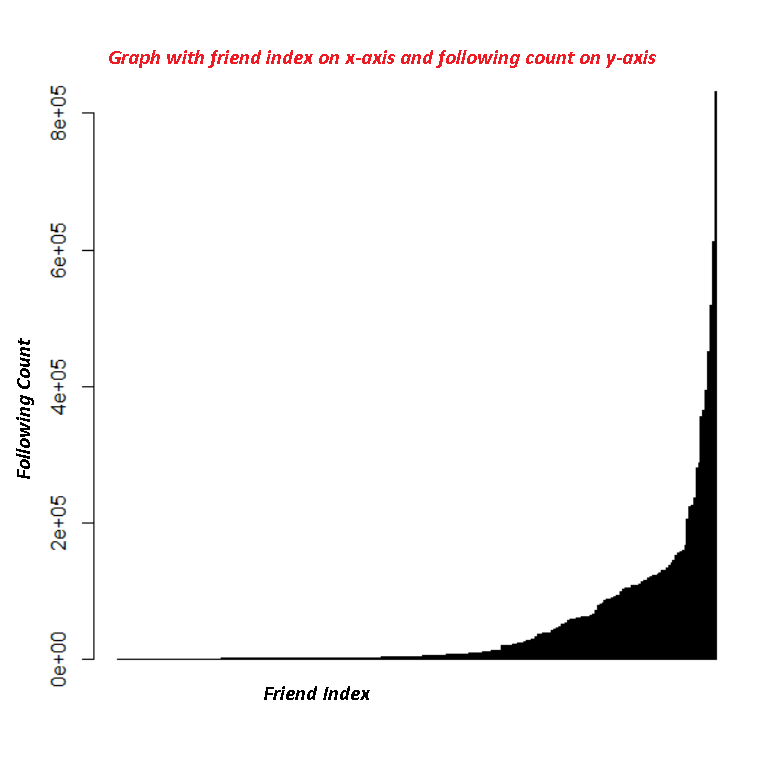
\includegraphics[scale=0.55, keepaspectratio=true]{figures/followingWithoutLog.PNG}
\caption{Graph with following count on y-axis and the friend index on x-axis }
\label{fig:q4fig2}
\end{center}
\end{figure}
\newpage
\item From the calculated median value `4609.5' and following count of `ohttic' `1,923' we can say that `ohttic' have less following count than his friends.
\ref{fig:q4fig2}.
\begin{figure}[h!]
\begin{center}
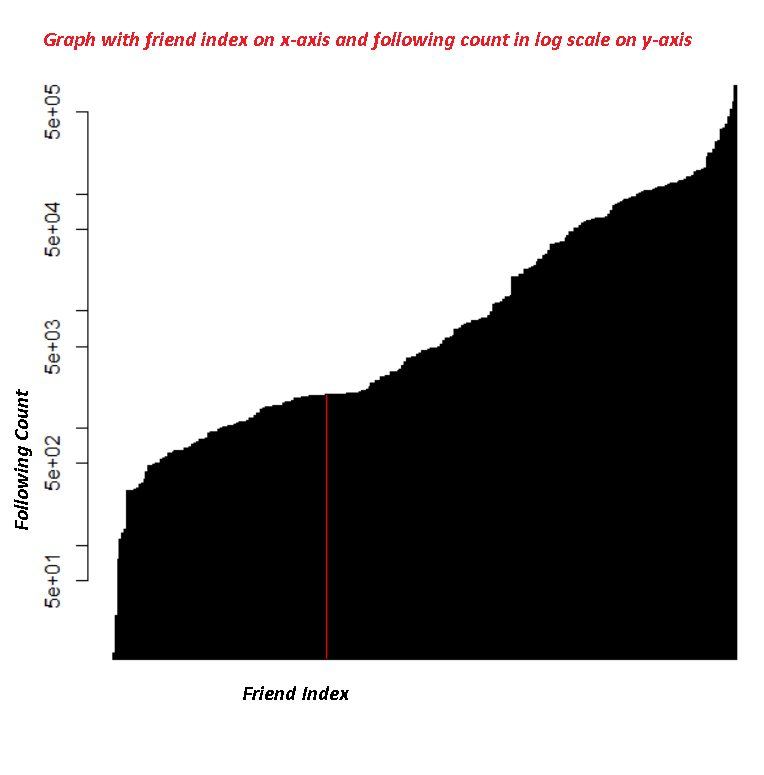
\includegraphics[scale=0.55, keepaspectratio=true]{figures/following.PNG}
\caption{Graph with following count in log scale on y-axis and the friend index on x-axis }
\label{fig:q4fig3}
\end{center}
\end{figure}
\end{itemize}

\newpage
\textbf{Code Listing}
\lstinputlisting[language=Python,caption=Python code for extracting friends count from JSON structure,frame=single,label=lst:q4code1,breaklines=true,captionpos=b,numbers=left,showspaces=false,showstringspaces=false,basicstyle=\footnotesize]{src/extractFollowing.py}

\textbf{Code Listing}
\lstinputlisting[language=Python,caption=Python code for calculating mean median and standard deviation,frame=single,label=lst:q4code2,breaklines=true,captionpos=b,numbers=left,showspaces=false,showstringspaces=false,basicstyle=\footnotesize]{src/getMeanMedianStandardDeviation3.py}


\backmatter
\bibliographystyle{ieeetr} 		
\nocite{*}  					
\small  					

 \bibliography{Master}

\end{document}